\chapter{Dodatek A}
\label{cha:appa}

\section{Oryginalny plik kml}
\label{sec:akml}

\lstset{language=XML}
\begin{lstlisting}[caption=caption]
<?xml version="1.0" encoding="UTF-8"?>
<kml>
  <Document>
    <name><![CDATA[US States]]></name>
    <open>1</open>
    <Style id="Style_5">
      <LabelStyle>
        <color>9900ffff</color>
        <scale>1</scale>
      </LabelStyle>
      <LineStyle>
        <color>990000ff</color>
        <width>2</width>
      </LineStyle>
      <PolyStyle>
        <color>997f7fff</color>
        <fill>1</fill>
        <outline>1</outline>
      </PolyStyle>
    </Style>
    <Placemark id="pm251">
      <name><![CDATA[Hawaii (1959)]]></name>
      <Snippet maxLines="0">empty</Snippet>
      <description></description>
      <TimeSpan>
        <begin>1989</begin>
      </TimeSpan>
      <styleUrl>#Style_5</styleUrl>
      <MultiGeometry>
        <MultiGeometry>
          <Polygon id="g867">
            <altitudeMode>clampToGround</altitudeMode>
            <outerBoundaryIs>
              <LinearRing>
                <coordinates>
-159.335174733889,21.9483433404175
-159.327130348878,22.0446395507162
-159.295025589769,22.1248124949548
-159.343195828355,22.1970166285359
-159.391366885913,22.2291198667724
-159.576012589057,22.2131796383001
-159.712505933171,22.1490592515515
-159.800814224332,22.0366665967853
-159.736592652746,21.9644203111023
-159.640246973766,21.9483657695954
-159.576021285803,21.8841361312636
-159.439545188912,21.8680716835921
-159.335174733889,21.9483433404175
                </coordinates>
              </LinearRing>
            </outerBoundaryIs>
          </Polygon>
        </MultiGeometry>
      </MultiGeometry>
    </Placemark>
  </Document>
</kml>

\end{lstlisting}

\section{Zapis w pamięci sesyjnej}
\label{sec:ass}

\lstset{language=XML}
\begin{lstlisting}[caption=caption]
[{"start":"1989","end":"2010","polygon":[{"lat":21.9483433404175,"lon":-159.335174733889},{"lat":22.0446395507162,"lon":-159.32713034887797},{"lat":22.1248124949548,"lon":-159.295025589769},{"lat":22.1970166285359,"lon":-159.34319582835496},{"lat":22.2291198667724,"lon":-159.391366885913},{"lat":22.2131796383001,"lon":-159.57601258905697},{"lat":22.1490592515515,"lon":-159.71250593317097},{"lat":22.0366665967853,"lon":-159.800814224332},{"lat":21.9644203111023,"lon":-159.73659265274603},{"lat":21.9483657695954,"lon":-159.640246973766},{"lat":21.8841361312636,"lon":-159.576021285803},{"lat":21.8680716835921,"lon":-159.439545188912},{"lat":21.9483433404175,"lon":-159.335174733889}],"title":"Hawaii (1959)","mId":"pm251","pId":"g867","color":"#ff0000","width":2,"opacity":0.59765625,"fillcolor":"#ff7f7f","name":"Hawaii (1959)","desc":""}]
\end{lstlisting}

\section{Wynik końcowy}
\label{sec:aresult}

\begin{figure}[H]
  \centering
    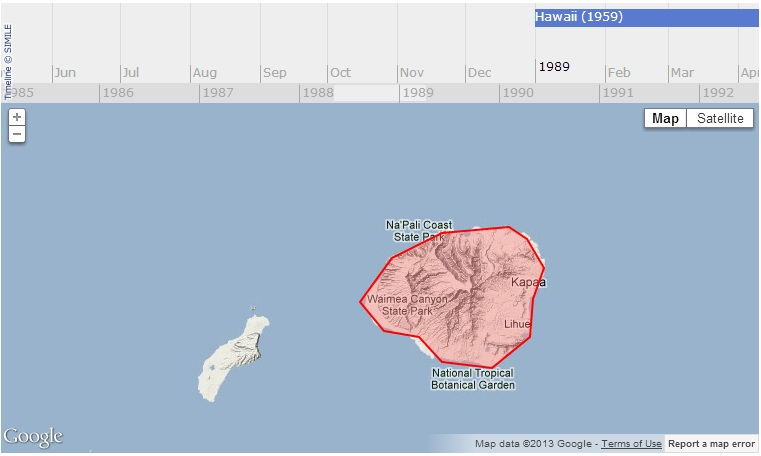
\includegraphics[width=100mm]{ge/hawaii.jpg}
  \caption{Hawaje}
  \label{fig:hawaii}
\end{figure}